\chapter{Industrialization, Testing, and Operational Readiness}

\section*{Introduction}
A distributed application is incomplete if it can only be explained from source code. Repeatable builds, controlled deployment, metrics, logs, traces, and explicit verification limits are part of the engineering result. This chapter evaluates the artifacts available in the three Qatra repositories.

\section{Repository and Delivery Organization}
The project is divided into three extracted repository folders:

\begin{itemize}
  \item \texttt{qatra-master}: donation service, notification service, PostgreSQL resources, Compose orchestration, CI and deployment workflows;
  \item \texttt{qatra\_angular-master}: Angular frontend, environment-generation script, Docker and Nginx resources, frontend workflow;
  \item \texttt{qatra\_infra-master}: k3s manifests using Traefik routing, plus Prometheus, Grafana, Loki, Promtail, Jaeger, and administration resources.
\end{itemize}

This separation supports different delivery concerns, but release compatibility must be managed. API changes, image tags, environment variables, and manifest versions should be coordinated rather than assuming every latest image is compatible.

\section{Continuous Integration}
The backend CI workflow runs for pull requests to the configured branches. A matrix creates one job for each service, installs Temurin Java 21 with Maven caching, and executes the Maven wrapper tests. This provides isolation: a failure identifies the affected service while keeping the workflow definition concise.

The local Windows inspection found a Maven wrapper startup error before tests could execute. The error occurred in the generated wrapper's PowerShell logic while accessing a filesystem target property. This report therefore records test inventory and CI intent but does not present local passing results.

\section{Continuous Deployment}
The deployment workflow responds to changes on the master branch. A path filter determines which service changed. The corresponding job authenticates to GHCR, builds and pushes a Docker image, connects to the server by SSH, imports the image into k3s, tags it for the local runtime, and restarts the deployment.

\diagram[0.41\textheight]{cicd-pipeline}{Qatra CI/CD pipeline from change to k3s rollout}

The workflow demonstrates automated deployment intent. Production hardening should add immutable version tags, rollout status verification, post-deployment health tests, and rollback to a known image. A restart alone does not prove that the new pods became ready or that business workflows remain valid.

\section{Container and Configuration Management}
The root Compose configuration defines the local distributed environment. Validation of the Compose model succeeded when syntax was checked, but numerous required environment variables were unset without an environment file. These include database credentials, JWT secrets, service URLs, Grafana credentials, and notification provider settings. This is expected for a template-driven repository, but setup documentation must make it explicit.

Secrets must not be committed in Compose or Kubernetes manifests. Example environment files should contain names and safe placeholders only. Production secrets should be supplied through a controlled mechanism and rotated when exposure is suspected.

\section{k3s Deployment}
The infrastructure manifests place the two application services and their operational dependencies in the single \texttt{qatra} namespace. Traefik \texttt{IngressRoute} resources expose the APIs and WebSocket endpoint; Nginx is used only by the local Compose topology. Deployment order matters: namespace and stateful dependencies precede application workloads; metrics/logging backends precede dashboards; ingress follows services.

The provided \texttt{deploy.sh} represents an operator entry point. A robust procedure should verify context and namespace, apply manifests declaratively, wait for readiness, and display failing pods or events. Administrative tools such as pgAdmin, RedisInsight, and Kubernetes Dashboard require strong access controls and should not be exposed publicly by default.

\section{Observability Architecture}
\begin{figure}[H]
\centering
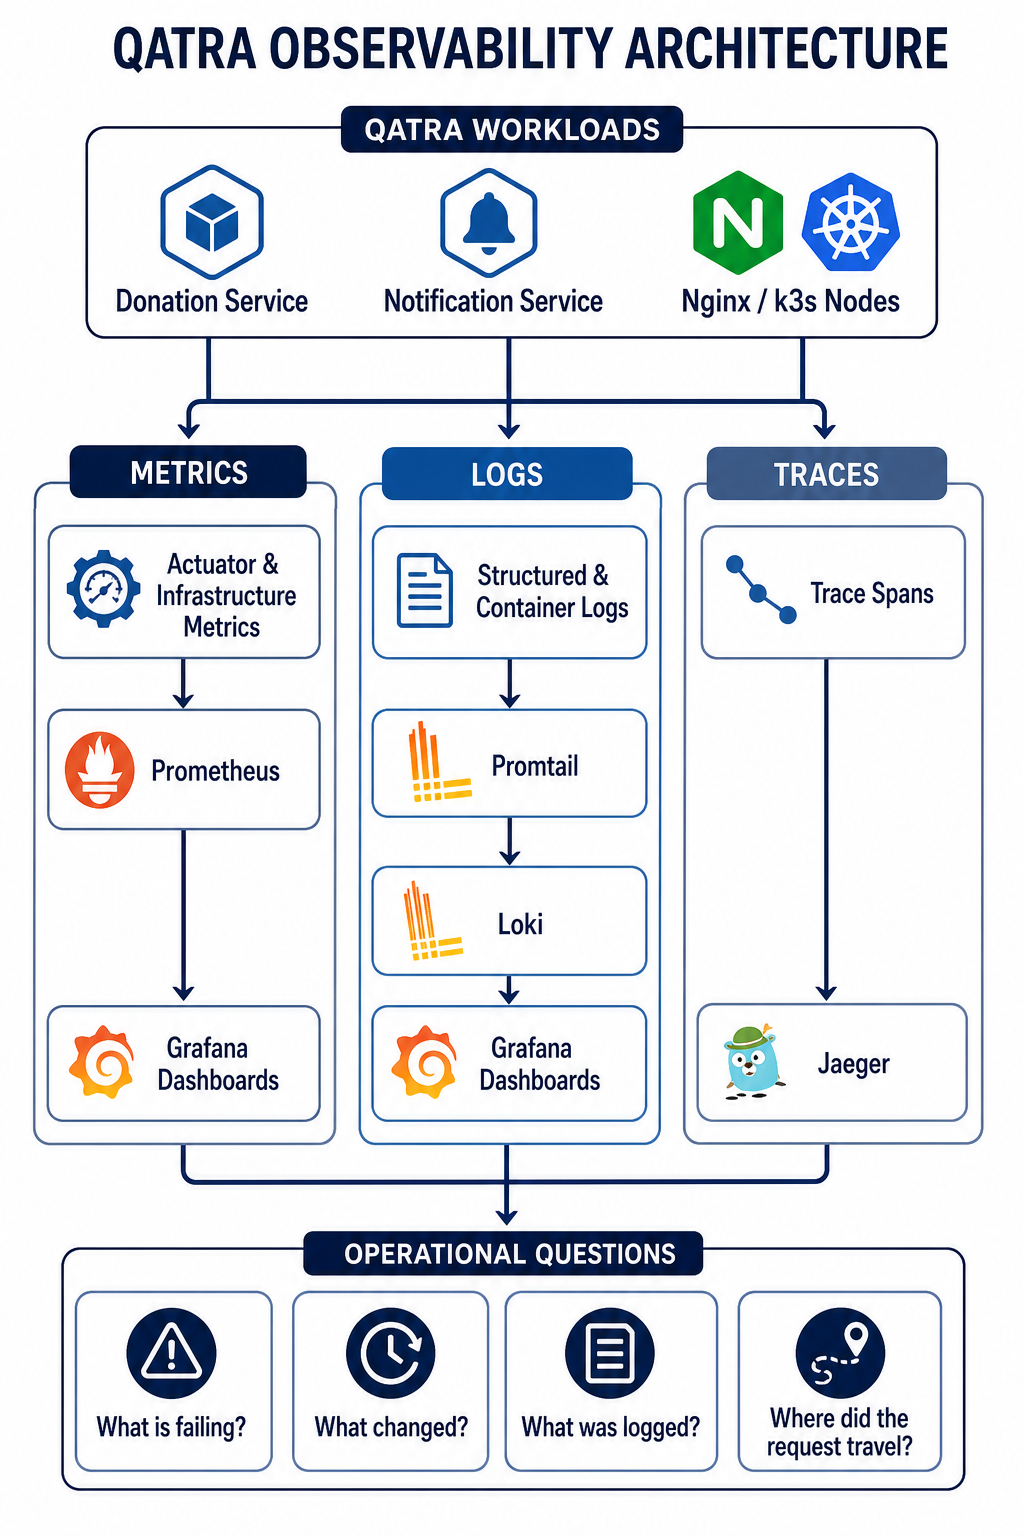
\includegraphics[width=0.82\textwidth,height=0.75\textheight,keepaspectratio]{assets/generated/observability-portrait.png}
\caption{Metrics, logs, and traces in the Qatra environment}
\label{fig:observability}
\end{figure}

Prometheus collects time-series data and makes it available to Grafana dashboards. Loki stores logs shipped by Promtail. Jaeger visualizes traces across service boundaries. These signals should share service, environment, instance, and correlation labels. High-cardinality values such as user IDs or raw URLs should not become metric labels.

Useful service-level indicators include request rate, error rate, latency, JVM memory, thread pools, database connection pools, Kafka consumer lag, notification retry count, WebSocket connections, and emergency matching duration. The repository contains monitoring configuration and dashboards; this report does not invent measured values from an unavailable running environment.

\section{Automated Test Inventory}
Static inspection identified 31 Java test files in the donation service, six Java test files in the notification service, and one Angular specification file. The count refers to files, not necessarily individual test methods. It demonstrates significant backend-oriented test structure and a clear frontend coverage gap.

\begin{table}[H]
\centering
\begin{tabularx}{\textwidth}{|P{4.1cm}|P{2.3cm}|Y|}
\hline
\rowcolor{tableheader}\textbf{Component} & \textbf{Test files} & \textbf{Interpretation}\\ \hline
Donation service & 31 & Domain/application/web checks are present; execution was blocked locally by wrapper startup\\ \hline
Notification service & 6 & Service-focused test structure exists; execution was blocked locally by the same wrapper issue\\ \hline
Angular frontend & 1 & Test infrastructure exists, but feature coverage is insufficient for the application size\\ \hline
\end{tabularx}
\caption{Observed automated test-file inventory}
\label{tab:test-inventory}
\end{table}

\subsection{Reproducibility Verification Performed for This Report}
The commands in Table~\ref{tab:verification-attempts} were executed in the supplied Windows workspace in August 2026. A failed prerequisite or wrapper startup is reported as such and is not counted as a failed application test.

\begin{table}[H]
\centering\small
\begin{tabularx}{\textwidth}{|P{3.4cm}|P{4.3cm}|Y|}
\hline
\rowcolor{tableheader}\textbf{Check} & \textbf{Observed evidence} & \textbf{Conclusion}\\ \hline
Java runtime & OpenJDK 21.0.11 was detected & Required backend runtime is available\\ \hline
Backend tests & \texttt{mvnw.cmd -B test} stopped in the wrapper's PowerShell bootstrap with a null-array error & Maven never started; no backend test pass or failure is claimed\\ \hline
Frontend production build & Angular reported a missing application-builder package because dependencies were not installed & Compilation did not start; no successful frontend build is claimed\\ \hline
CI definition & GitHub Actions matrix targets donation-service and notification-service with Java 21 and Maven tests & Workflow intent is verified; no exported run result was available\\ \hline
k3s deployment & Manifests define one \texttt{qatra} namespace, Traefik routes, two application services, and operational dependencies & Static deployment topology is verified; no live rollout result is claimed\\ \hline
\end{tabularx}
\caption{Reproducible checks and their observed outcomes}
\label{tab:verification-attempts}
\end{table}

\section{Recommended Test Strategy}
\subsection{Domain and Unit Tests}
Pure domain tests should cover compatibility, eligibility dates, appointment transitions, emergency transitions, tier expansion, ranking, and reliability bounds. These tests are fast and should avoid Spring context startup.

\subsection{Persistence and Integration Tests}
Repository adapters should be tested against PostgreSQL-compatible behavior, including constraints, pagination, and concurrent slot updates. Kafka integration tests should verify serialization, consumer behavior, duplicate handling, and retry classification. Testcontainers is a suitable future approach for reproducible dependencies.

\subsection{API and Security Tests}
Controller tests should verify validation, error contracts, role enforcement, ownership, and filtering of sensitive fields. Negative cases are essential: a valid token with the wrong center scope must be rejected.

\subsection{Frontend Tests}
The Angular application needs unit tests for stores, services, schemas, guards, and critical components. End-to-end tests should cover registration, login, onboarding, appointment booking, staff completion, emergency creation, donor response, and administrative approval. Browser tests must use isolated data and should not depend on real email providers.

\subsection{Operational Tests}
Deployment verification should include Compose configuration, Kubernetes schema checks, image scanning, startup health, database connectivity, Kafka connectivity, and a minimal API smoke test. Observability tests can verify that actuator metrics are scraped and that a correlated request produces searchable logs and a trace.

\section{Security and Production Readiness}
\begin{longtable}{|P{3.4cm}|P{4.8cm}|P{5.2cm}|}
\hline
\rowcolor{tableheader}\textbf{Area} & \textbf{Available foundation} & \textbf{Required hardening}\\ \hline
Authentication & Spring Security and JWT dependencies & Key rotation, revocation strategy, brute-force controls guided by OWASP API Security~\cite{owaspApiSecurity}\\ \hline
Authorization & Roles and protected application features & Systematic object- and resource-scope tests~\cite{owaspApiSecurity}\\ \hline
Secrets & Environment-driven configuration & Managed secrets, rotation, and leak scanning\\ \hline
Containers & Service Dockerfiles and registry workflow & Non-root images, SBOM, vulnerability scanning, immutable tags\\ \hline
Kubernetes & Namespaced manifests and ingress & Network policies, resource limits, pod security, backup tests\\ \hline
Data & PostgreSQL persistence and GDPR workflows & Encryption, minimization, retention policy, restore drills, legal review~\cite{gdpr}\\ \hline
Events & Kafka infrastructure & Schema governance, idempotency, dead-letter operation\\ \hline
Observability & Metrics, logs, traces, dashboards & Alerts, retention, PII redaction, on-call procedures\\ \hline
\caption{Production-readiness foundation and hardening roadmap}
\label{tab:readiness}
\end{longtable}

\section{Problems Encountered and Corrective Directions}
\subsection{Build Reproducibility}
The Maven wrappers use script-only distribution bootstrap. In the inspected Windows environment, the generated PowerShell logic fails before Maven starts. Corrective options are to update the wrapper, add the wrapper JAR distribution mode, or execute in the Linux CI environment. The correct fix should be verified in both services.

\subsection{Frontend Dependency Setup}
The frontend includes a lock file but no installed \texttt{node\_modules} directory, which is normal for a clean source archive. A reproducible setup should use the lock file and a supported Node version. The build script generates development and production environment files before Angular compilation.

\subsection{Environment Completeness}
Compose configuration is structurally valid but depends on variables. A setup checklist should copy the example file, supply secure values, verify ports, and confirm external notification credentials. Validation must ensure placeholders are not accepted in production.

\subsection{Evidence Gaps}
The source archive contains no application screenshots and no exported CI execution history. The report therefore uses labeled screenshot placeholders and describes workflow configuration without fabricated screenshots or pass rates. This makes the remaining documentation work explicit and preserves academic integrity.

\section{Improvement Roadmap}
Short-term priorities are repairing the Maven wrapper, expanding Angular tests, adding API smoke tests, and capturing controlled UI evidence. Medium-term priorities are transactional event publication, schema governance, immutable deployments, backups, alerting, and security scanning. Longer-term work could include validated demand forecasting, hospital-system integration, mobile clients, accessibility testing, and real-world usability evaluation under appropriate governance.

\section*{Conclusion}
Qatra includes a credible industrialization foundation: CI and deployment workflows, containers, k3s manifests, and a complete observability stack. At the same time, local build limitations, frontend test scarcity, and missing execution evidence prevent exaggerated claims. This distinction between implemented foundation and verified result is essential for responsible engineering reporting.
